\section{International adoption}
\label{sec:Adoption}

\subsection{European Union}

\subsubsection{Developments since the IFRS's adoption}
Over 100 countries now use IFRS. These accounting standards have been increasingly discussed at international level (e.g. G20, Basel Committee) and with various interested parties in the EU, especially in the wake of the financial crisis. \\

Several initiatives concerning technical issues and governance are under way, both internationally and in the EU. \\

In the EU, the reform of European Financial Reporting Advisory Group (EFRAG) which advises the Commission on IFRS matters was successfully implemented on 31 October 2014 when the amended statutes and internal rules of EFRAG came into force. These changes, based on the recommendations from the report of Mr Maystadt, are designed to strengthen the EU’s contribution to achieving high accounting standards globally. 


\subsubsection{Commission evaluation}
The Commission is evaluating the IAS Regulation assessed whether:
\begin{itemize}
	\item the Regulation achieved its objective in an efficient and effective manner;
	\item the criteria that all new IFRS should meet to become EU law are appropriate and whether the process for adoption of standards works properly;
	\item the governance structure of the bodies developing the standards and advising the Commission is appropriate.
\end{itemize}

The Commission conducted the evaluation based on the following sources and workstreams:
\begin{itemize}
	\item a public consultation,
	\item an informal expert group,
	\item the Accounting Regulatory Committee (ARC) which comprises representatives of all Member States,
	\item a review of the literature on the impact of the mandatory adoption of IFRS in the EUpdf Choose translations of the previous link and on the performance of IFRS during the crisispdf Choose translations of the previous link,
	\item internal experience of relevant international and European bodies,
	\item Philippe Maystadt’s recommendations.
\end{itemize}

The key findings showed that IFRS was successful in creating a common accounting language for capital markets. Companies were mostly positive about their experience of using IFRS and in most cases, benefits outweighed costs. Investors also largely supported IFRS for improving the transparency and comparability of financial statements. Most stakeholders considered that the process through which IFRS become part of EU law works well. Importantly, the recent reform of the European Financial Reporting Advisory Group (EFRAG), which is the technical advisor to the Commission in this field, will strengthen the EU voice in the international standard-setting process. \\

The report identifies room for improvement in some areas. The collaboration between actors in the endorsement process could be enhanced to improve timeliness and to allow for a more holistic consideration of standards with other aspects of EU law. IFRS issued by the IASB need to be endorsed by the Commission. An endorsement process remains necessary to ensure that the standards developed by a private body meet certain criteria and are fit for the European economy before becoming part of EU law.

\subsection{United States of America}
The U.S. is moving toward IFRS. Unlike what happened with other countries, IASB and FASB have been working on convergence for many years. \\

By the end of the ’90s, the two predominant standards were the U.S. GAAP (Generally Accepted Accounting Principles) and IFRS. And, both standard setters, IASB and FASB (Financial Accounting Standards Board), initiated a convergence project even before IFRS was actually adopted by many countries. \\

\subsubsection{Principle Based vs. Rule Based}
One of the major differences lies in the conceptual approach: U.S. GAAP is rule-based, whereas IFRS is principle-based. \\

The inherent characteristic of a principles-based framework is the potential of different interpretations for similar transactions. This situation implies second-guessing and creates uncertainty and requires extensive disclosures in the financial statements. \\

In a principle-based accounting system, the areas of interpretation or discussion can be clarified by the standards-setting board, and provide fewer exceptions than a rules-based system. However, IFRS include positions and guidance that can easily be considered as sets of rules instead of sets of principles. At the time of the IFRS adoption, this led English observers to comment that international standards were really rule-based compared to U.K. GAAP that were much more principle-based. \\

The difference between these two approaches is on the methodology to assess an accounting treatment. Under U.S. GAAP, the research is more focused on the literature whereas under IFRS, the review of the facts pattern is more thorough. \\

However, the professional judgment is not a new concept in the U.S. environment. The SEC is addressing this topic in order to find the right balance between the “educated” professional judgment, that is acceptable, and the “guessed” professional judgment. \\

\subsubsection {Differences Between IFRS and U.S. GAAP}
While this is not a comprehensive list of differences that exist, these examples provide a flavor of impacts on the financial statements and therefore on the conduct of businesses.
\begin{itemize}
	\item \textbf{Consolidation} — IFRS favors a control model whereas U.S. GAAP prefers a risks-and-rewards model. Some entities consolidated in accordance with FIN 46(R) may have to be shown separately under IFRS.
	\item \textbf{Statement of Income} — Under IFRS, extraordinary items are not segregated in the income statement, while, under US GAAP, they are shown below the net income.
	\item \textbf{Inventory} — Under IFRS, LIFO (a historical method of recording the value of inventory, a firm records the last units purchased as the first units sold) cannot be used while under U.S. GAAP, companies have the choice between LIFO and FIFO (is a common method for recording the value of inventory).
	\item \textbf{Earning-per-Share} — Under IFRS, the earning-per-share calculation does not average the individual interim period calculations, whereas under U.S. GAAP the computation averages the individual interim period incremental shares.
	\item \textbf{Development costs} — These costs can be capitalized under IFRS if certain criteria are met, while it is considered as “expenses” under U.S. GAAP.

	\item \textbf{Balance Sheet} - The primary difference between a U.S. GAAP balance sheet and an IFRS balance sheet is in the order of presentation. U.S. GAAP financial statements follow an order of liquidity reporting structure, with a careful delineation between current and non-current assets and liabilities. This means the most liquid assets are reported first in the current asset section of a balance sheet and liabilities requiring the most immediate cash in the coming year are reported in the current liabilities sections of the balance sheet. IFRS do not specify the balance sheet format or structure. The guidelines simply say the balance sheet must show the entity’s assets, liabilities and equities. A company is not required to list assets or liabilities in order of liquidity but is required to specify each section of assets and liabilities as current and noncurrent.
\end{itemize}

\begin{figure}[h]
\caption{Analysis by Nature of Expense (IRFS)}
\centering
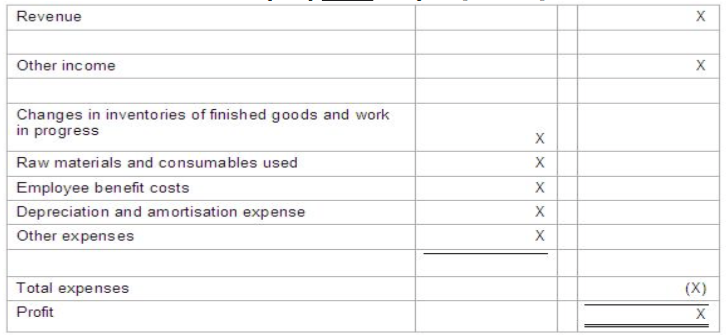
\includegraphics[width=0.8\textwidth]{images/natureOfExpenses.png}
\end{figure}

\begin{figure}[h]
\caption{Analysis by Function of Expense (GAAP)}
\centering
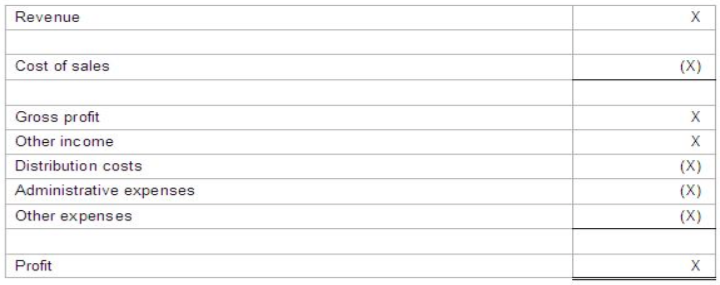
\includegraphics[width=0.8\textwidth]{images/functionOfExpenses.png}
\end{figure}

\clearpage
\subsection{Effect on Income}
In many areas, IFRS is less conservative than U.S. GAAP, meaning that it allows an increase in the risk of overstating income in a company’s financial statements. IFRS also allows more flexibility than U.S. GAAP, and since bonus and stock option schemes usually give managers incentives to increase income, this flexibility likely will be used to increase income more often than it will be used to decrease income. It is important to note that income is always an estimate, based on management judgments such as the useful life of long-term assets, the expected losses from bad debts, the expected costs of warranties, and the diminution of large assets such as the value of equipment and the value of accounting goodwill. It can be argued that the income estimate under U.S. GAAP has no more intrinsic validity than the estimate under IFRS. However, setting aside the question of intrinsic validity, it is fairly clear that switching from U.S. GAAP to IFRS will lead to many companies reporting higher income numbers, even while holding cash flows constant. European companies quoted on U.S. markets provide a natural laboratory since they were required to report in both U.S. GAAP and IFRS until very recently. Citigroup London analyzed 73 of the largest European companies quoted in the U.S. and found that 82 percent of the firms reported higher income under IFRS than under U.S. GAAP.

\subsection{Effect on Investors}
Looking at these findings, the adoption of IFRS would seem like great news for investors. But this is not the case. Remember, these European companies were reporting two different income figures based on the same financial year, that is, based on the same economic activity and cash flows. The question of which income number is the “true” estimate of underlying profit is irrelevant to some extent. Investors used to analyzing U.S. GAAP income will have to adjust and discount IFRS figures: one additional dollar of IFRS profit indicates slightly lesser incremental economic health and, if the underlying assumptions of accounting are accepted, slightly lesser ability to pay down debt and pay dividends in the future than one dollar of income calculated under U.S. GAAP.

Apart from magnitude, the second useful facet of income numbers is change. Earnings volatility, often minimized by earnings management techniques that are legally dubious, is an important signal to investors of a company’s underlying health. Annual income numbers should reflect the economic performance of the company in that particular year. The pre-IFRS GAAP of many European countries often allowed companies wide latitude to manage earnings and show a smooth pattern of earnings change from year to year that hid changes in company performance investors may have wanted disclosed. Although IFRS has substantially changed those practices, more latitude remains than under U.S. GAAP. This has a deleterious effect on how useful IFRS reports are to shareholders. Research shows that European companies’ IFRS reports, although more informative than pre-IFRS GAAP reports, are less informative than U.S. GAAP reports for the same firms, because IFRS reports show smoother earnings, show less correlation between reported earnings and cash flow, show less timely loss recognition, and crucially, show less association between reported earnings and firms’ stock prices.


\subsection{Why adopt IRFS?}
Today, the world’s  nancial markets are borderless. Companies (including small companies) seek capital at the best price wherever it is available. Investors and lenders seek investment opportunities wherever they can get the best returns commensurate with the risks involved. To assess the risks and returns of their various investment opportunities, investors and lenders need  nancial information that is relevant, reliable and comparable across borders. \\

The amounts of cross-border investment are enormous. To illustrate:
\begin{itemize}
	\item the Organisation for Economic Co-operation and Development (OECD) estimates that worldwide Foreign Direct Investment (FDI) out ows in 2013 were US\$1.281 trillion. The historically highest level was in 2007 (US\$2.170 trillion).
	\item cross-border ownership of stocks and bonds amounts to many trillions of US dollars. For example, foreign ownership of US equities, corporate bonds and treasuries amounted to nearly US\$14 trillion in 2013. And US investors held over US\$9 trillion of foreign corporate stocks and bonds in 2013.
\end{itemize}

The use of one set of high quality standards by companies throughout the world improves the comparability and transparency of  nancial information and reduces  nancial statement preparation costs. When the standards are applied rigorously and consistently, capital market participants receive higher quality information and can make better decisions.
Thus, markets allocate funds more ef ciently and  rms can achieve a lower cost of capital.
A comprehensive review of nearly 100 academic studies of the bene ts of IFRS concluded that most of the studies ‘provide evidence that IFRS has improved ef ciency of capital market operations and promoted cross-border investment’.




















